\begingroup
\small
\begin{frame}
\frametitle{Методы восстановления}
\begin{tabular}{p{0.15\textwidth} | p{0.4\textwidth} | p{0.4\textwidth}}
\hspace{-1cm} семейство & Интегральные & Алгебраические \\ \hline \vspace{10pt}
\hspace{-1cm} подход & формула для обращения $R^{-1}[p(\varphi, \xi)](x,y)$ & Оптимизационная задача $\min_{f} \Norm{R[f] - p}$\\ \hline \vspace{5pt}
\hspace{-1cm} представители & \footnotesize{Filtered Backprojection (FBP)} & \footnotesize{Algebraic Reconstruction Technique (ART),\ Simultaneous ART (SART),\ Simultaneous Iterative RT (SIRT) }\\ \hline \vspace{3pt}
\hspace{-1cm} сложность & $O(N^2 \log N)$ & $O(N^3)$ \\ \hline \vspace{5pt}
\hspace{-1cm} особенности & универсальность & возможность учета модели объекта или \\
                          & требует полного набора проекционных углов, их равномерного распределения  & измерительной схемы \\ 
                          & чувствительны к шумам & \\
\end{tabular}
\\
\vspace{3pt}
$N$ --- число ячеек детектора
\end{frame}
\endgroup

\begin{frame}
\frametitle{Метод Свертки и обратной проекции}
\begin{columns}
  \hspace{-0.1cm}
  \begin{column}{0.6\textwidth}
    Основные шаги метода:
    \begin{itemize}
    \item Фильтрация проекций: $\tilde{p}(\xi, \varphi) = \mathscr F ^{-1}[|u| \mathscr F[p(\xi, \varphi)](u)]$\\
    $\mathscr F[\cdot], \mathscr F ^{-1}[\cdot]$ --- прямое и обратное преобразования Фурье по $\xi$\\
    \vspace{10pt}
    \item Вычисление обратной проекции $f(x,y) = \int_0^\pi {\tilde{p} (x \cos\varphi + y \sin \varphi, \varphi) d\varphi}$
    \end{itemize}
  \end{column}

  \begin{column}{0.6\textwidth}
  Достоинства:
  \begin{itemize}
    \item скорость работы
    \item универсальность
    \item точная формула (при непрерывных значениях $\xi, \varphi$)
  \end{itemize}
  Недостатки:
  \begin{itemize}
    \item требует равномерную сетку углов
    \item чувствителен к шумам
    \item не позволяет учитывать специфики эксперимента
  \end{itemize}
  \end{column}
\end{columns}
\end{frame}

\begin{frame}
\centering
\frametitle{Метод Свертки и обратной проекции}
  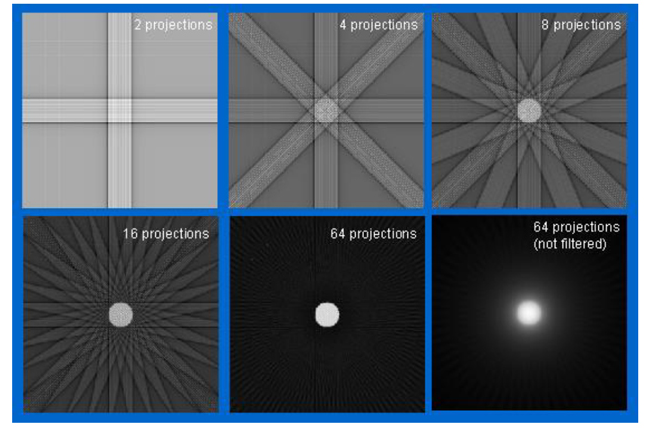
\includegraphics[width=0.8\textwidth]{fbp_img.png}
  \\
  Операция обратной проекции
\end{frame}

%\section{Вычислительно эффективный алгебраический метод восстановления FHT-SIRT}

\begin{frame}
\frametitle{Алгебраический метод}
\framesubtitle{Основные положения}
\begin{itemize}
  \item непрерывные функции $\rightarrow$ дискретные изображения:

    {
    \centering
    $f(x,y) \rightarrow f_i,\ p(\varphi, \xi) \rightarrow p_j$
    \par
    }
  \vspace{0.5cm}
  \item преобразование Радона $\rightarrow$ преобразование Хафа:
  
    {
    \centering
    $R[f](\varphi, \xi) \rightarrow (\mathrm W f)_j$ 
    \par
    }
  \vspace{0.5cm}

    $\mathrm W$ --- матрица проекции, указывает вклад пикселя $i$ в лучевую сумму вдоль луча $j$.\\
    Разреженная матрица размера $N_\varphi * N^3$, в которой только порядка $O(N_\varphi * N^2)$ ненулевых элементов
    \vspace{0.5cm}
  \item решение разреженной СЛАУ большой размерности итерационным методом

    {
    \centering
    $p = \mathrm W f$
    \par
    }

\end{itemize}
\end{frame}

\begin{frame}
\frametitle{Матрица проекции W}
\begin{tabular}{c c c}
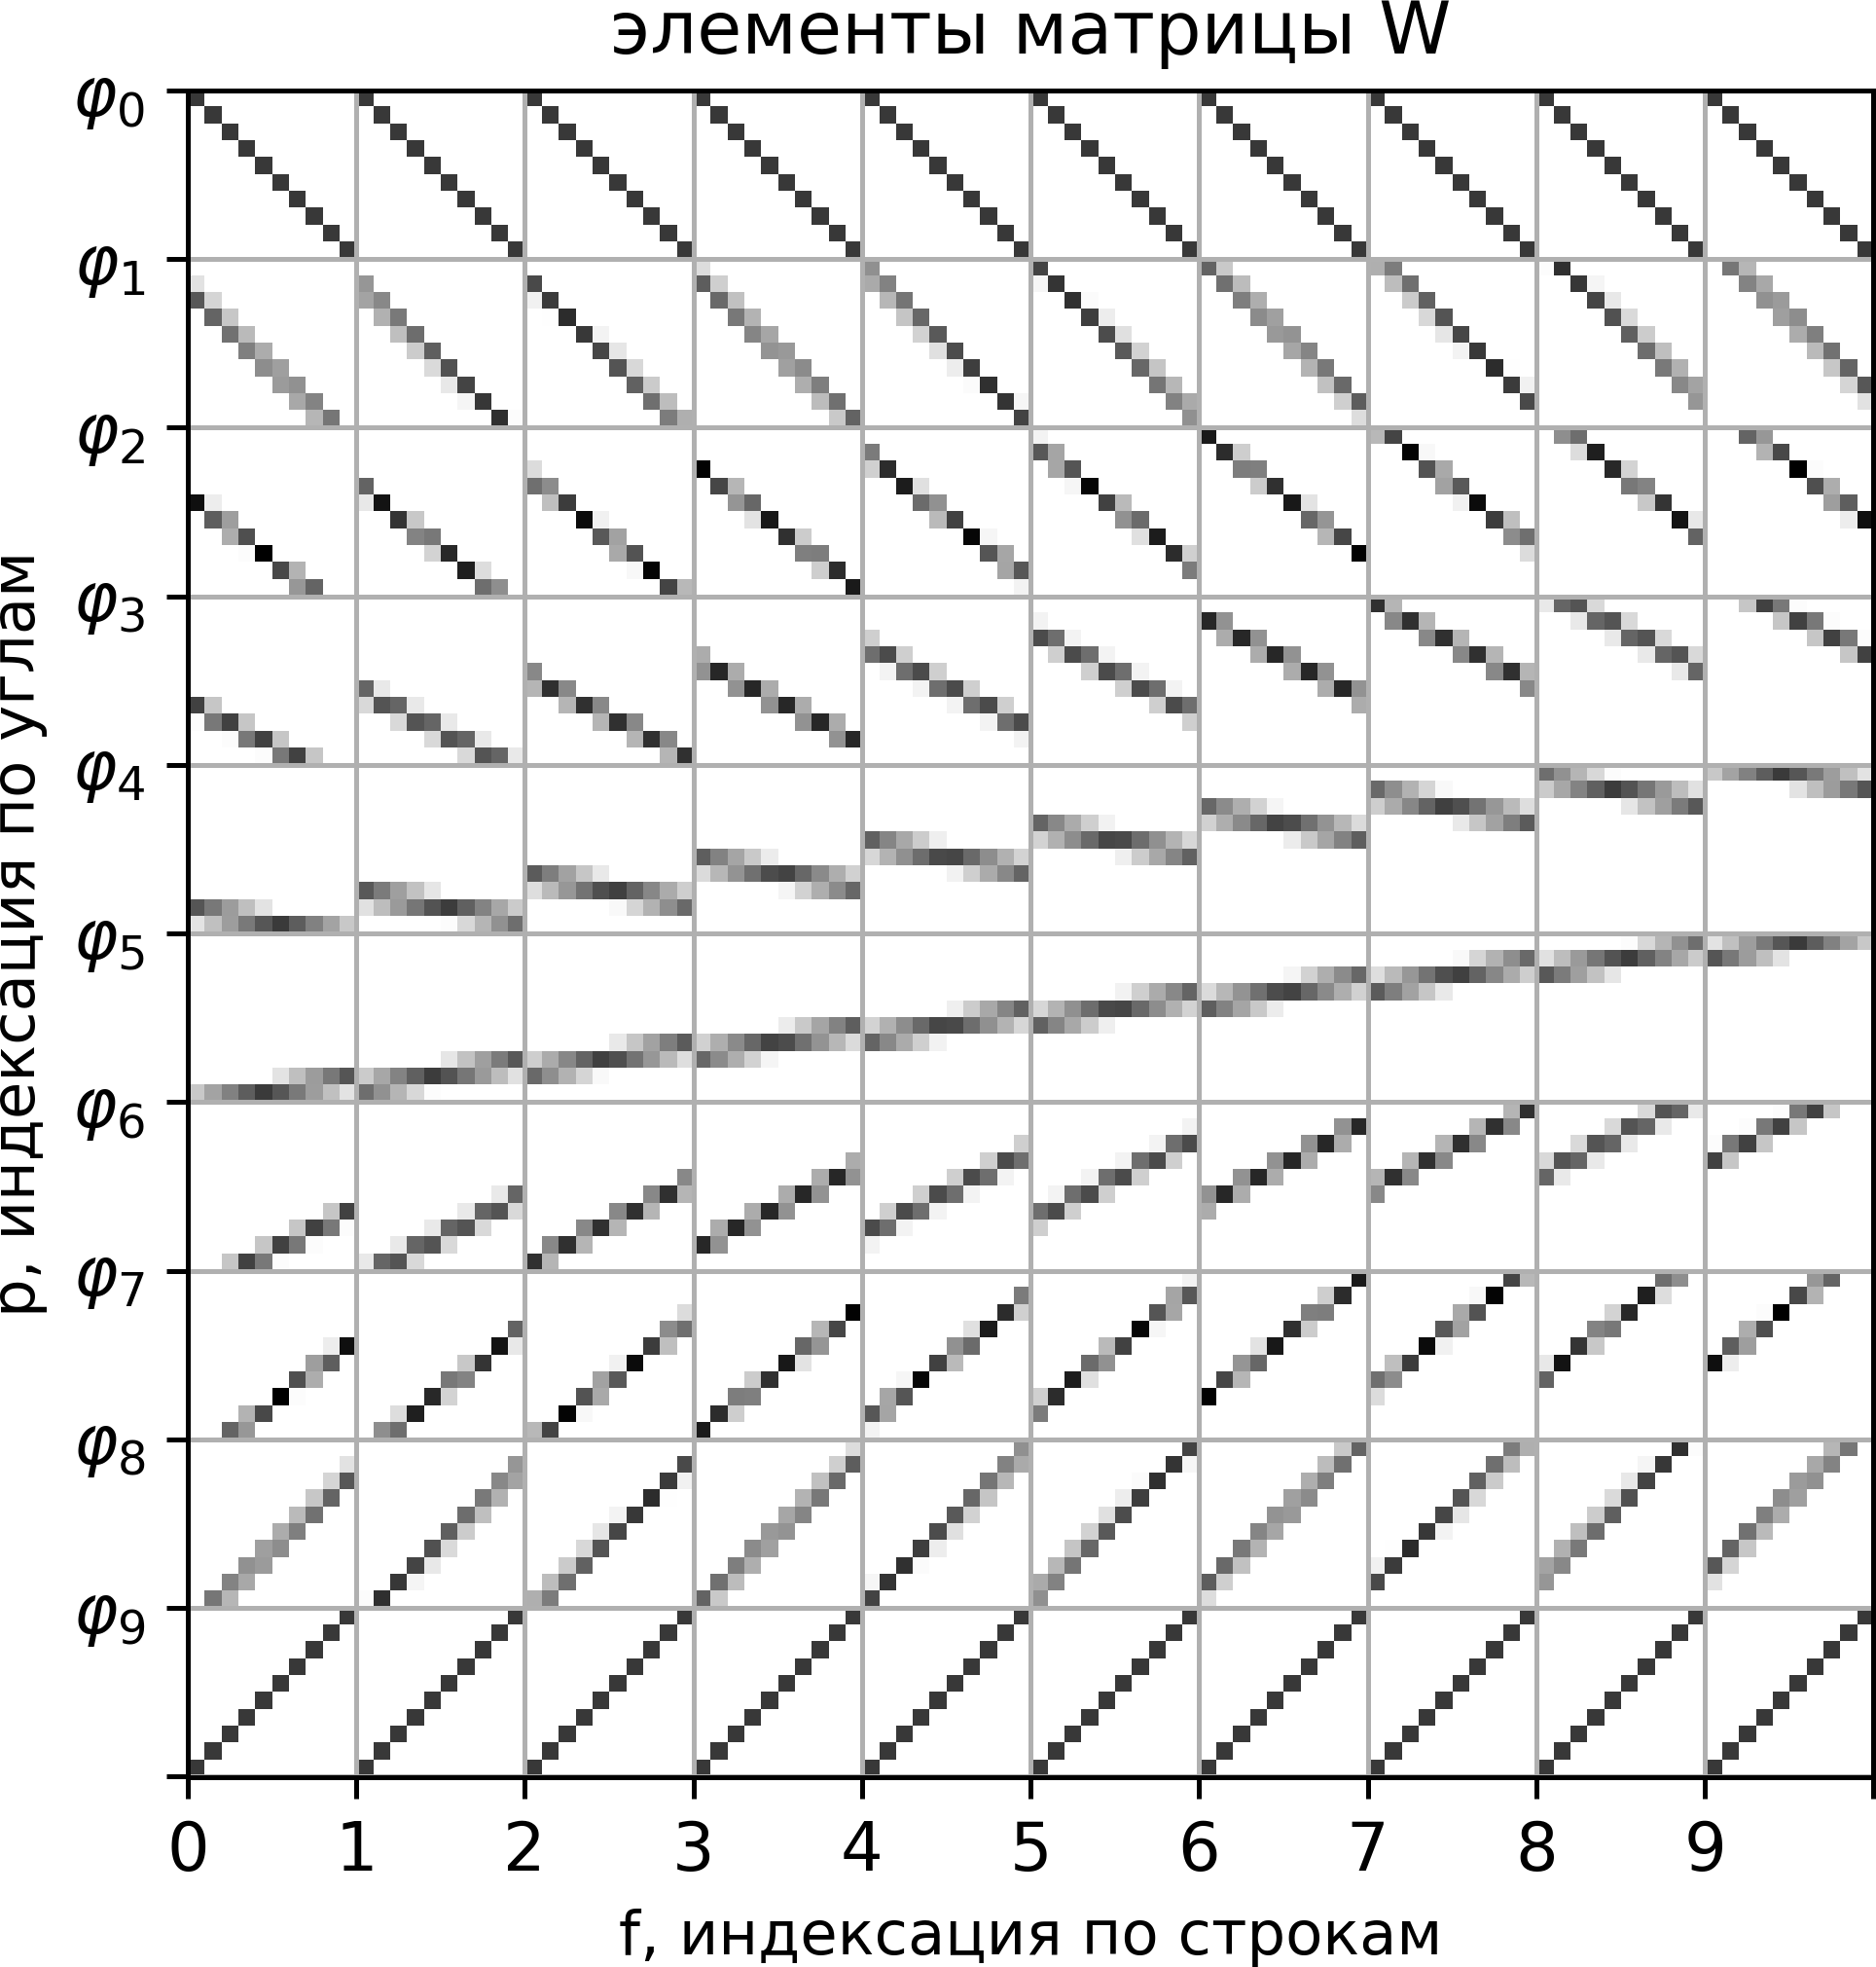
\includegraphics[width=0.4\textwidth]{w_matrices/W_10_10_plot.png} &
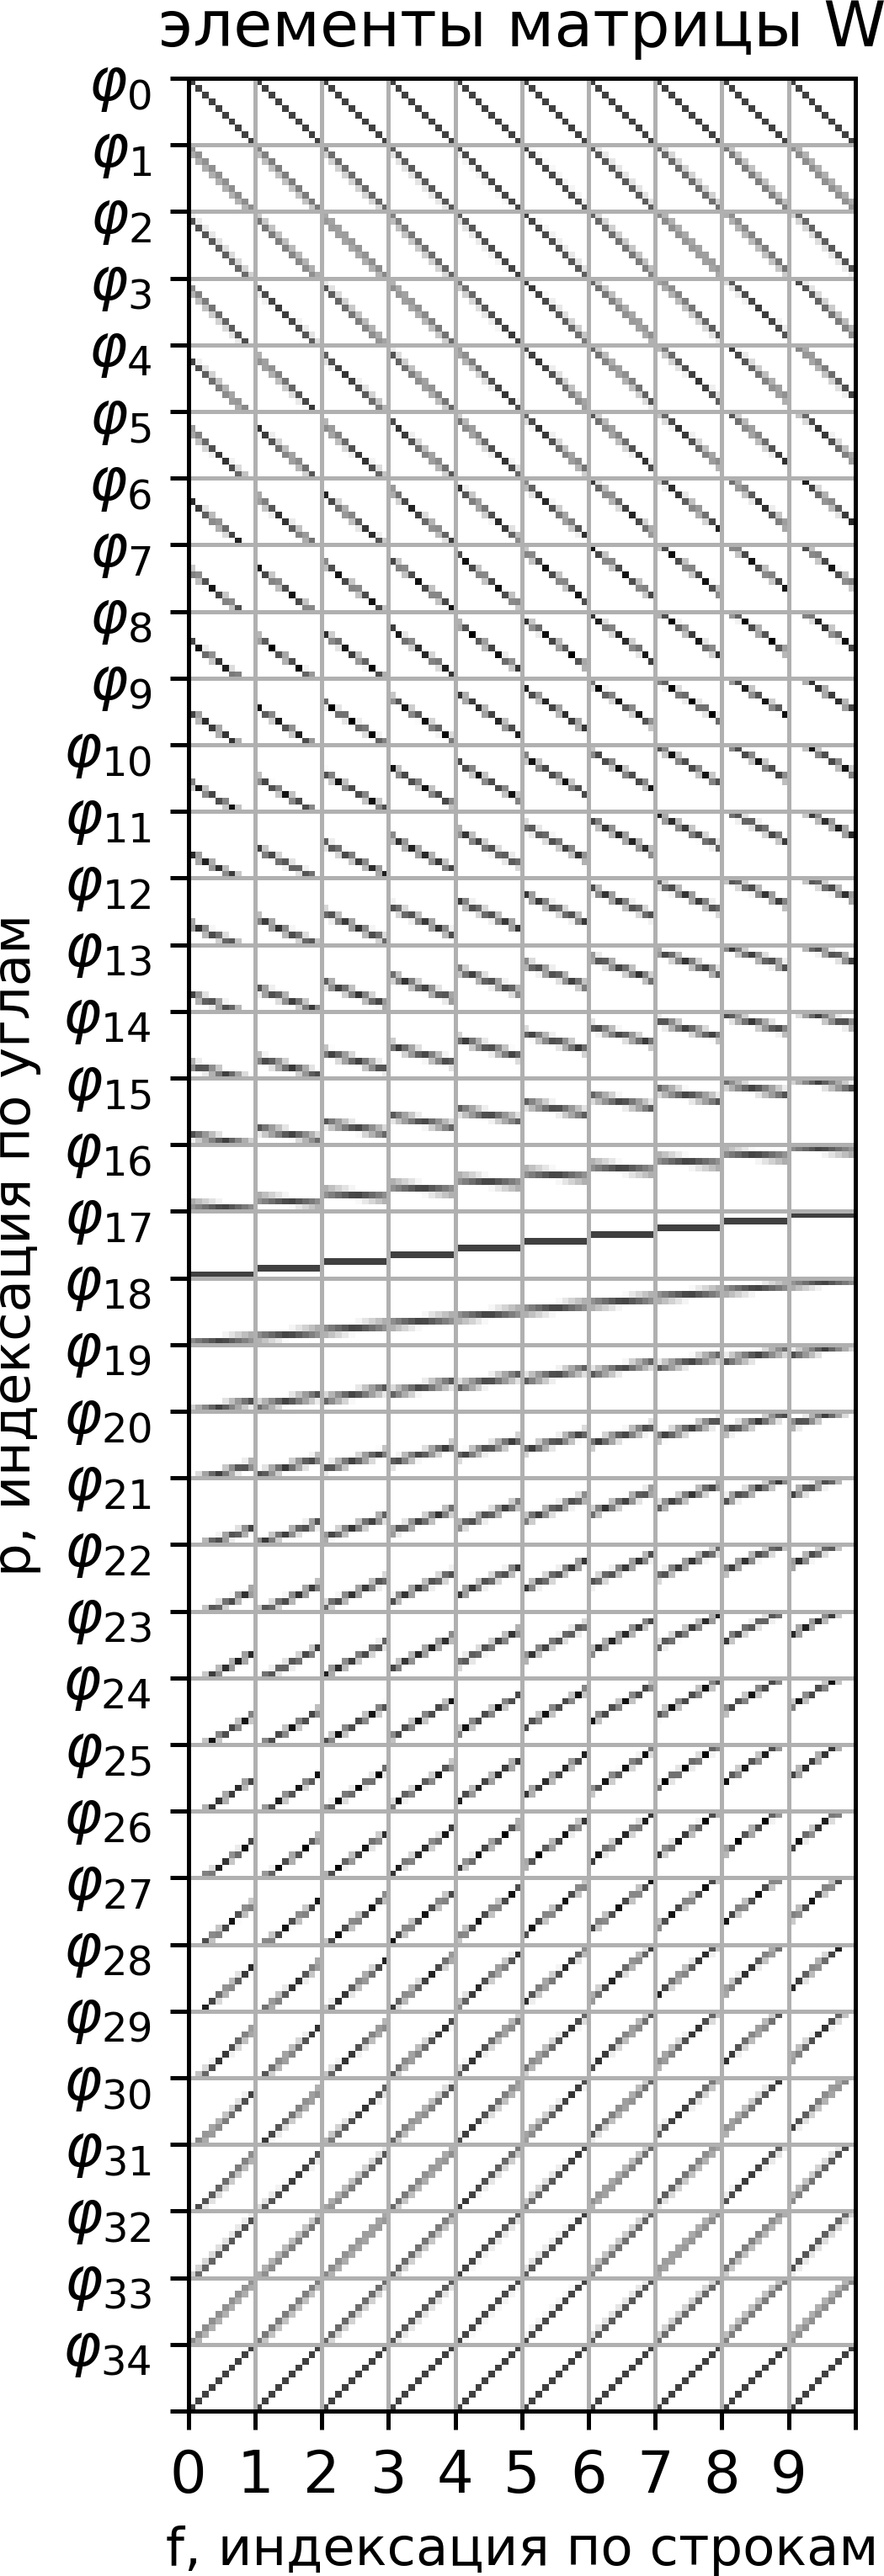
\includegraphics[height=0.8\textheight]{w_matrices/W_10_35_plot.png} &
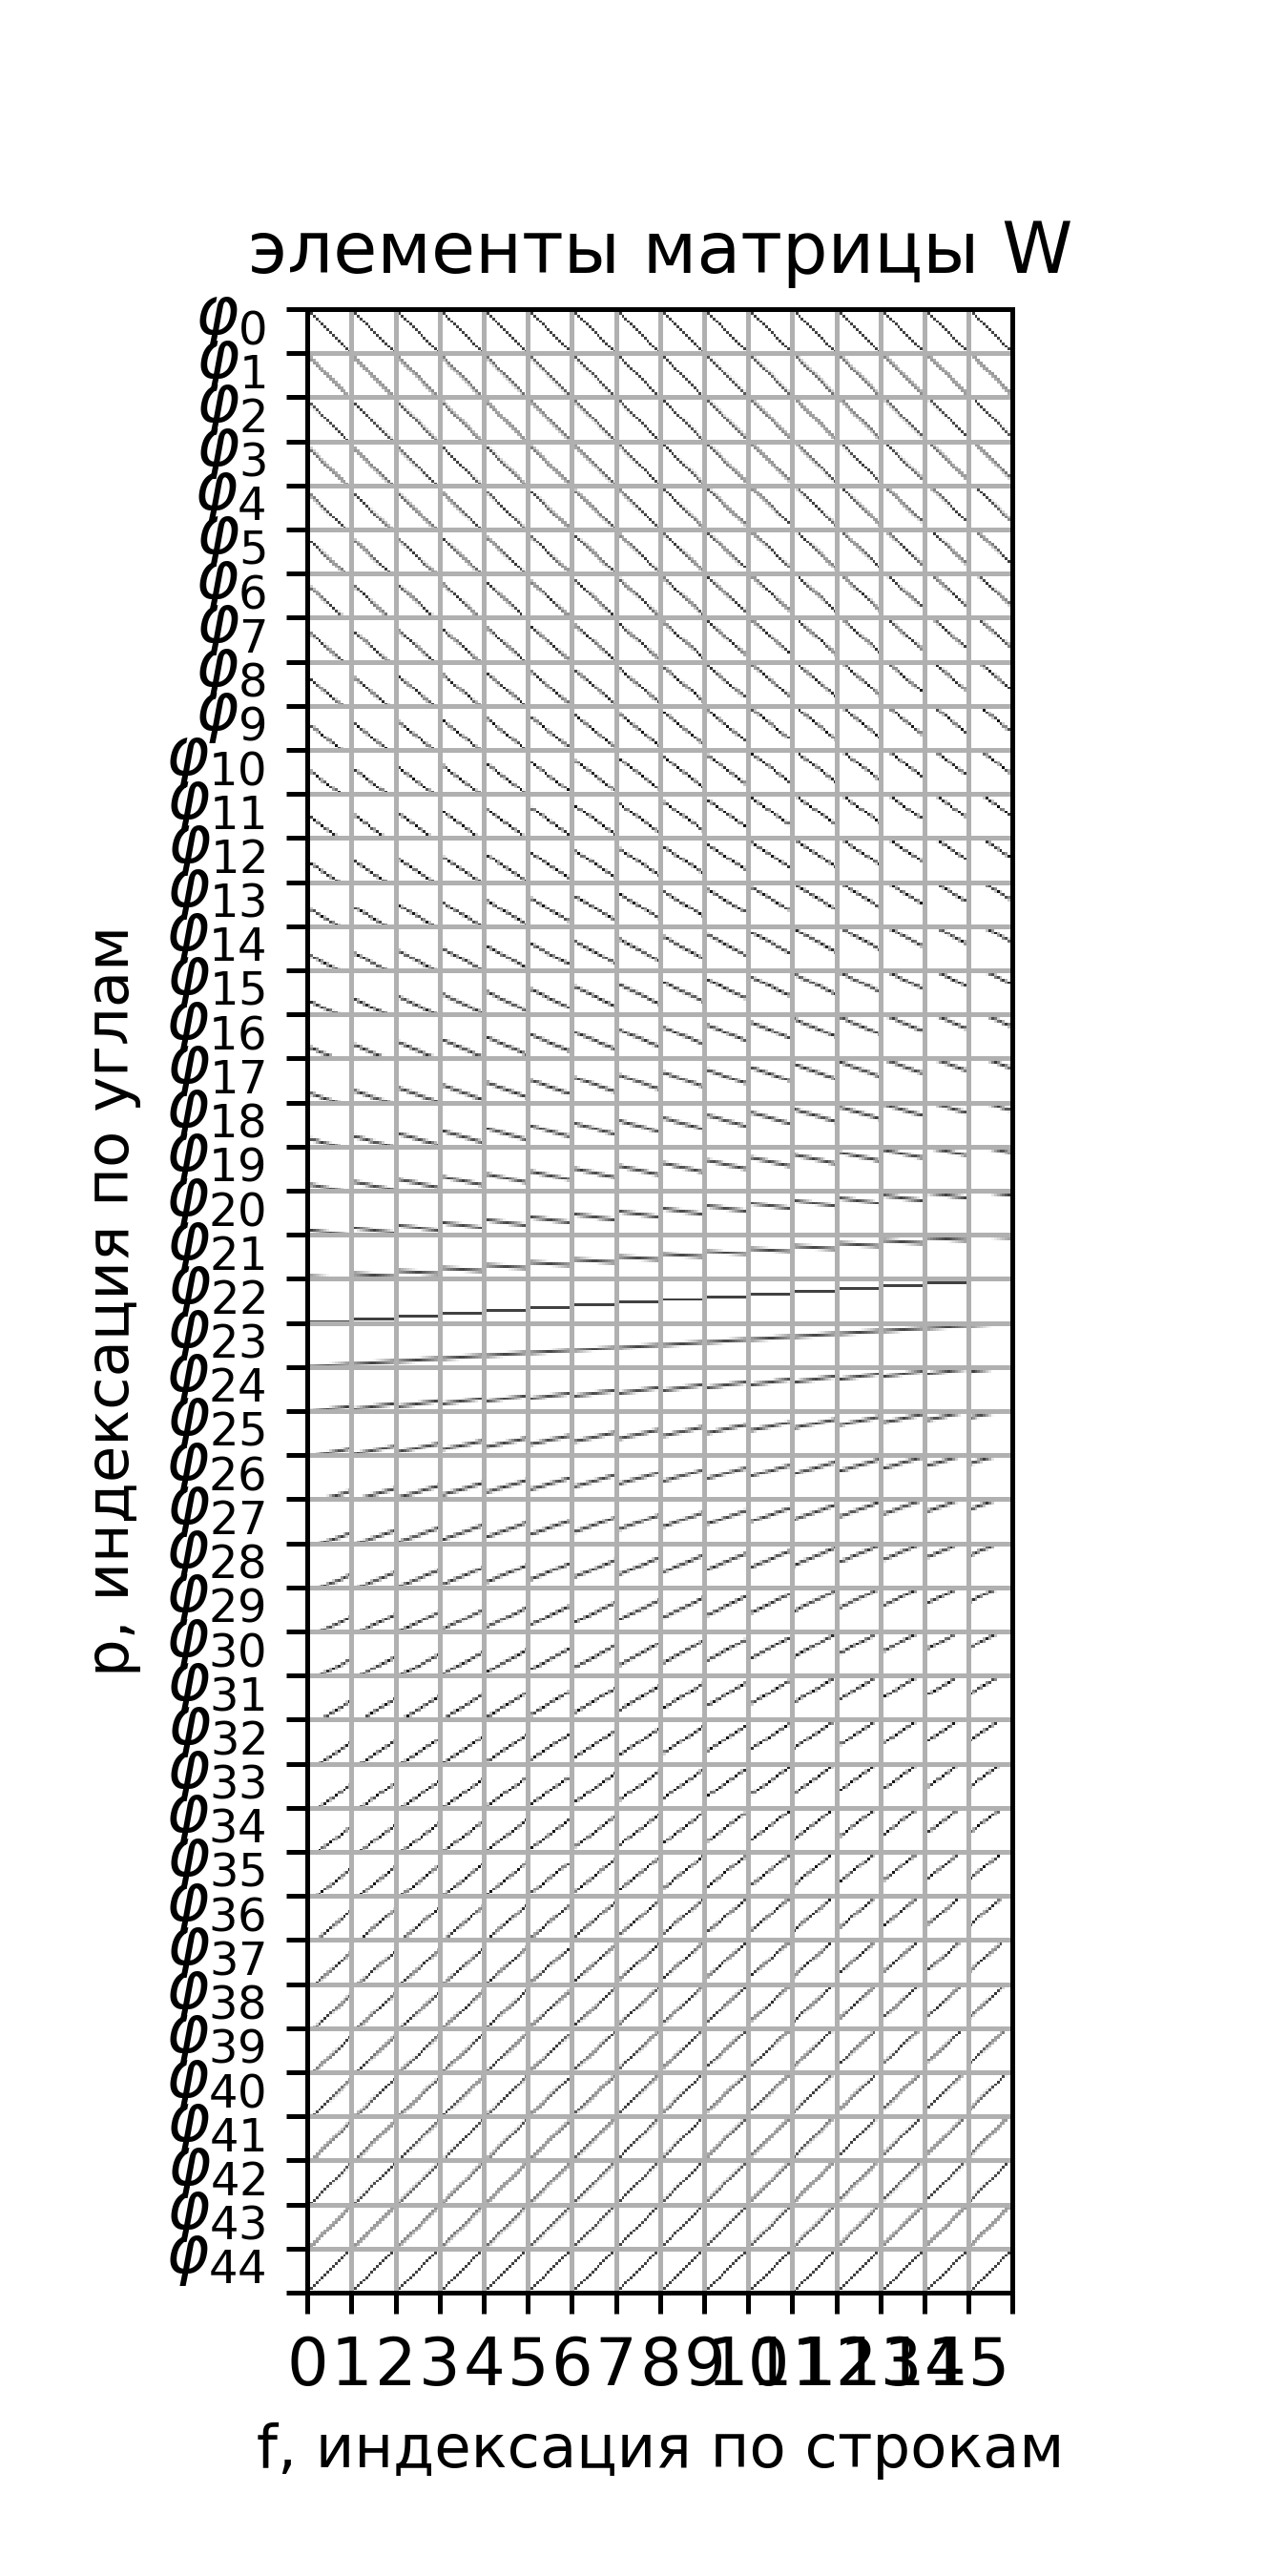
\includegraphics[height=0.8\textheight]{w_matrices/W_16_45_plot.png} \\
\small{$N = 10$, $N_\varphi = 10$} &
\small{$N = 10$, $N_\varphi = 35$} & 
\small{$N = 16$, $N_\varphi = 45$}
\end{tabular}
\end{frame}

\begin{frame}
\frametitle{Алгебраический метод}
\framesubtitle{Решение СЛАУ}
\centering
$\Norm{p - \mathrm W f} \rightarrow \min\limits_f$

Оптимизационная задача решается итерационным методом, шаг итерации имеет вид
\vspace{0.5cm}

\begingroup
\footnotesize

\hspace*{-0.5cm}
\begin{tabular}{c|c|c}
ART & SART & SIRT \\ \hline
для каждого луча & для каждого угла & для всех лучей\\
$j = 1 \dots N * N_\varphi$ & $\varphi_k$ & \\
$\hat{f} = f - \gamma \mathrm W^{\mathrm T}_j(\mathrm W f - p)$ &
$\hat{f} = f - \gamma \mathrm {W^{\varphi_k}}^{\mathrm T}(\mathrm W f - p)$ &
$\hat{f} = f - \gamma \mathrm W^{\mathrm T}(\mathrm W f - p)$ \\
\end{tabular}

\vspace{0.2cm}
\raggedright
\endgroup

$\mathrm W_j$ --- столбец матрицы для луча $j$,\\
$\mathrm W^\varphi$ ---  матрица проекции на угол $\varphi$, $\mathrm W = \sum_\varphi {\mathrm W^\varphi}$
\\
\vspace{0.4cm}

$\mathrm W f$ --- прямая проекция, \\
$\mathrm W^{\mathrm T} p$ --- обратная проекция.
\end{frame}


\begin{frame}
\frametitle{SIRT}
\framesubtitle{Анимация процесса восстановления}
\begin{columns}[T,onlytextwidth]
\begin{column}{0.4\textwidth}
\animategraphics[loop,controls,width=\linewidth]{10}{anim/frame_}{1}{60}
\end{column}

\begin{column}{0.6\textwidth}
\animategraphics[loop,controls,width=\linewidth]{10}{anim/slice_}{1}{60}
\end{column}
\end{columns}
%\endgroup
\end{frame}

\begin{frame}
\frametitle{Алгебраический метод}

Преимущества:\\
\begin{itemize}
  \item качество восстановления
  \item возможность учета специфики эксперимента (регуляризация, ограничения)
\end{itemize}
\vspace{1.5cm}

Недостатки:\\
\begin{itemize}
  \item сложность настройки
  \item низкая скорость работы
  \item сходимость
\end{itemize}
\end{frame}

\begin{frame}
\frametitle{Направления развития алгебраических методов}

\begin{itemize}
  \item \textbf{ускорение}
  \begin{itemize}
    \item использование GPU
    \item \textbf{улучшение асимптотики итерации}
    \item ускорение сходимости итерационной процедуры
  \end{itemize}
  \item \textbf{улушчение качества восстановления, борьба с артефактами}
    \begin{itemize}
    \item огрубление луче (beam hardening)
    \item \textbf{артефакты из-за сильнопоглощающих включений (metal artifacts)}
    \end{itemize}
  \item \textbf{учет спектра источника} \\
  \small{В условиях лабороторного спектра восстановленная характеристика является усреднением линейного коэффициента полгощения по спектру. Это затрудняет интерпретацию результатов восстановления. }
\end{itemize}

\end{frame}